%%%%%%%%%%%%%%%%%%%%%%%%%%%%%%%%%%%%%%%%%%%%%%%%%%%%%%%%%%%%%%%%%%%%%%
% Lớp 12 | Ứng dụng đạo hàm để khảo sát hàm số | Khảo sát sự biến thiên và vẽ đồ thị hàm số
% Dạng 2D1?5-7: Điểm đặc biệt của đồ thị hàm số
% Số câu: 31  (sinh tự động bởi tach_cau.py; từ nay thầy sửa trực tiếp file này)
%%%%%%%%%%%%%%%%%%%%%%%%%%%%%%%%%%%%%%%%%%%%%%%%%%%%%%%%%%%%%%%%%%%%%%

%%%%%%%%%%%%%%%% TRẮC NGHIỆM 4 PHƯƠNG ÁN %%%%%%%%%%%%%%%%

% nguồn: Phan1_Lop_12_Dai_so_Chuong_1
\begin{ex}%[2D1H5-7]%[ma:09375dd7]
	 \immini{
		Một trong bốn điểm sau đây là tâm đối xứng của đồ thị ở hình bên, diểm đó là điểm  nào?
	\choice 
			{\True $M\left(\dfrac{1}{2}; \dfrac{1}{2}\right)$} 
			{$N\left(1;  \dfrac{1}{2}\right)$}
			{$P\left(\dfrac{1}{2};  1\right)$}
			 {$O(0; 0)$
			 }
			 }{\resizebox{!}{5cm}{
			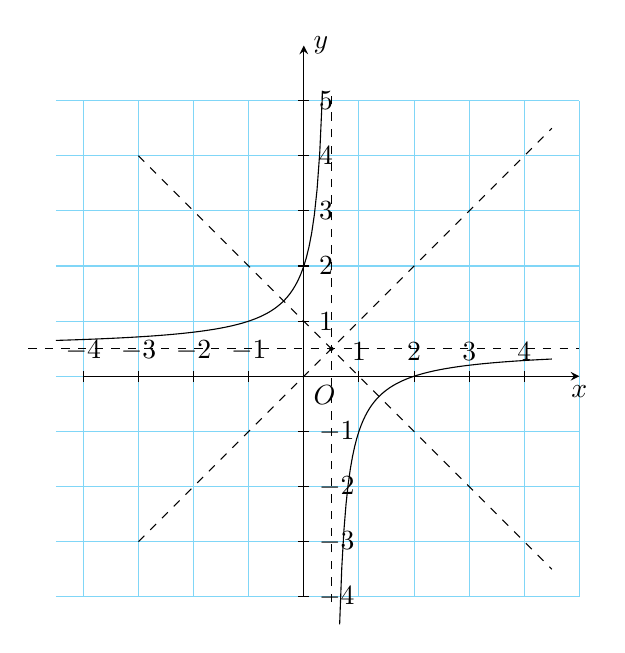
\begin{tikzpicture}[scale=0.7,>=stealth]
				\draw[cyan!50,thin] (-4.5,-4) grid  (5,5);
				 \draw[->] (-4,0)--(0,0)
					node[below  right]{$O$}--(5,0) node[below]{$x$};
				\draw[->] (0,-4)  --(0,6) node[right]{$y$};
				\foreach \x in  {-4,-3,-2,-1,1,2,3,4}{
					 \draw (\x,-.1)--(\x,.1) node[above]{$\x$};
				 }
				\foreach \y in {-4,-3,-2,-1,1,2,3,4,5}{ 
					\draw (-.1,\y)--(.1,\y)  node[right]{$\y$};
				} 
				\draw[samples=100,domain=-4.5:0.34]  plot (\x,{(\x-2)/(2*(\x)-1)});
				\draw[samples=100,domain=0.65:4.5] plot (\x,{(\x-2)/(2*(\x)-1)}); 
				\draw  [domain=-3:4.5,dashed] plot (\x,{(\x)});
				\draw  [dashed] (-5,0.5)--(5,0.5);
				 \draw [domain=-3:4.5,dashed] plot (\x,{(-\x+1)});
				\draw [dashed] (0.5,-4.1)--(0.5,5.1); 
				\draw[fill] (0.5,0.5)  circle (1pt);
			\end{tikzpicture}
			 }
			 }
	 \loigiai{
			Ta có thể lấy Tâm đối  xứng của đồ thị nếu có giao của $2$ tiệm cận rồi. Áp dụng bài này ta thấy điểm đó là $M\left(\dfrac{1}{2}; \dfrac{1}{2}\right)$.
		 }
	\end{ex}

% nguồn: Phan1_Lop_12_Dai_so_Chuong_1
\begin{ex}%[2D1H5-7]%[ma:7c35258a]
	\immini{Đồ thị như  hình vẽ là của hàm số
	\choice 
			{$y=x^3-x^2+x+1$} 
			{\True  $y=x^3-3x^2+3$}
			 {$y=x^3+3x^2+3x+1$}
			{$y=x^2+2x+1$} 
			}{\begin{tikzpicture}[scale=0.6,>=stealth,font=\footnotesize,line join=round,line cap=round]
		\def\a{1}  \def\b{-3} \def\c{0} \def\d{3}
		 \def\xmin{-2} \def\xmax{5}
		 \def\ymin{-2} \def\ymax{4}
		\draw[->] (\xmin,0)--(\xmax,0) node [below]{$x$}; 
		\draw[->] (0,\ymin)--(0,\ymax) node [left]{$y$}; 
		\node at (0,0) [below  left]{$O$};
		\clip (\xmin+0.1,\ymin+0.1) rectangle (\xmax-0.5,\ymax-0.1); 
		 \draw[smooth,samples=300] plot (\x,{\a*(\x)^3+\b*(\x)^2+\c*(\x)+\d});
	\end{tikzpicture}
			 }
	\loigiai{ 
			Dựa vào đồ thị ta có hàm số đã  cho là hàm số bậc 3 và có 2 cực trị nên $y=x^3-3x^2+3$.
		} 
	\end{ex}

% nguồn: Phan1_Lop_12_Dai_so_Chuong_1
\begin{ex}%[2D1H5-7]%[ma:772ba5b6]
	 \immini{
		Cho hàm số $y=f(x)$ có đồ  thị ở hình bên. Đường thẳng nào sau đây là trục đối xứng của đồ thị hàm số đã cho?
	\choice 
			 {$y=x$}
			{\True $y=-x$} 
			{$y=0$} 
			{$x=0$} 
			}{\resizebox{!}{5cm}{\begin{tikzpicture}[scale=0.6,>=stealth,line join=round,line cap=round]
		\draw[->] (-4,0)--(4,0) node[below]{$x$}; 
		\draw[->]  (0,-4)--(0,5) node[left]{$y$};
		\draw[samples=100,domain=-4:-1.5]  plot (\x,{((\x)-1)/((\x)+1)});
		\draw[samples=100,domain=-0.6:3.8] plot (\x,{((\x)-1)/((\x)+1)}); 
		 \draw[samples=100,domain=-4:4] plot (\x,{1});
		\draw[samples=100,domain=-4:5,smooth,variable=\y] plot ({-1},\y); 
		\draw (0,0) node[above  left]{$O$};
		 \draw[dashed]
			(-1,0) node[above  left]{$-1$}
			(0,-1) node[left]{$-1$} 
			(0,1)  node[above right]{$1$}
			(1,0) node[above]{$1$}; 
		\fill  (0,0) circle (1pt);
		\fill (0,1) circle  (1pt);
		 \fill (0,-1) circle (1pt);
		\fill (1,0) circle  (1pt);
	\end{tikzpicture}
			 }
			 }
	 \loigiai{
		 \immini{
			Ta có thể quan sát thấy tiệm cận  đứng của đồ thị hàm số là $x=-1$.\\
			Tiệm cận ngang của đồ thị hàm số là  $y=1$.
			Giao điểm  của hai đường tiệm cận là $(-1; 1)$.
			Đường thẳng $y=-x$ đi qua giao điểm của  hai tiệm cận. Do đó
			$y=-x$ là trục đối xứng  của đồ thị hàm số đã cho.\\
			Hoặc có thể dùng bút chì kẻ  các đường $y=x$, $y=-x$, $y=0$, $x=0$ và quan sát thì chỉ $y=-x$ thoả mãn là trục đối xứng của đồ thị hàm số đã cho.
			 }{
			\begin{tikzpicture}[scale=0.6,>=stealth,line join=round,line cap=round]
				 \path (0:0) coordinate (O);
				 \draw[->] (-4,0)--(4,0) node[below]{$x$};
				 \draw[->] (0,-4)--(0,5) node[left]{$y$};
				\draw[samples=100,domain=-4:-1.5]  plot (\x,{((\x)-1)/((\x)+1)});
				\draw[samples=100,domain=-0.6:3.8]  plot (\x,{((\x)-1)/((\x)+1)});
				 \draw[samples=100,domain=-4:4] plot (\x,{1});
				\draw[samples=100,domain=-4:4] plot (\x,{1}); 
				\draw[samples=100,domain=-4:4] plot (\x,{(\x)}) node[right]  {$y=x$};
				\draw[samples=100,domain=-4:4] plot (\x,{(-\x)})  node[right] {$y=-x$};
				\draw[samples=100,domain=-4:5,smooth,variable=\y] plot  ({-1},\y);
				 \draw[dashed]
					 (-1,0) node[above left]{$-1$}
					(0,-1)  node[left]{$-1$}
					(0,1) node[above right]{$1$} 
					(1,0)  node[above]{$1$};
				\fill (0,0)  circle (1pt);
				\fill (0,1) circle  (1pt);
				\fill (0,-1) circle (1pt); 
				\fill (1,0)  circle (1pt);
				\fill (-1,0)  circle (1pt);
				\fill (-1,1) circle  (1pt);
				\foreach \x/\g  in {O/110}
				\fill (\x) circle  (1pt)
					($(\g:7mm)+(\x)$) node  {$\x$};
			\end{tikzpicture}
		}} 
	\end{ex}

% nguồn: Phan1_Lop_12_Dai_so_Chuong_1
\begin{ex}%[2D1H5-7]%[ma:82def6b5]
		Đồ thị  của hàm số $y=\dfrac{x-2}{x+1}$ là
	\choice 
			{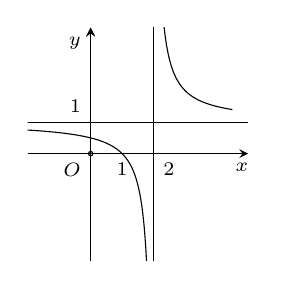
\begin{tikzpicture}[>=stealth,scale=0.4]
		\clip (-2,-3.4)  rectangle (6,4);
		 \draw[->,color=black] (-2,0.) -- (5,0.);
		\foreach  \x in {1,2}
		\draw[->,color=black]  (0.,-4) -- (0.,4);
		\draw  (2,-5)--(2,5)
			(-5,1)--(5,1); 
		\draw[smooth,samples=100,domain=-4.5:1.9]  plot (\x,{(\x-1)/(\x-2)});
		\draw[smooth,samples=100,domain=2.1:4.5] plot (\x,{(\x-1)/(\x-2)}); 
		\draw (0,1)  node[above left] {\scriptsize $1$};
		\draw (1,0) node[below] {\scriptsize  $1$};
		\draw (2,0) node[below right] {\scriptsize $2$}; 
		\draw (4.8,0) node[below]  {\scriptsize $x$};
		\draw (0,3.5) node[left] {\scriptsize  $y$};
		\draw (0,0) circle (2pt) node[below  left] {\scriptsize $O$};
	\end{tikzpicture}
			 }
			{\begin{tikzpicture}[>=stealth,scale=0.4]
		\clip (-5,-3)  rectangle (6,5);
		 \draw[->,color=black] (-5,0.) -- (3,0.);
		\draw[->,color=black] (0.,-3.4)  -- (0.,5);
		 \draw (-1,-5)--(-1,5)
			(-5,2)--(3,2); 
		 \draw[smooth,samples=100,domain=-4.5:-1.1] plot (\x,{(2*\x-2)/(\x+1)});
		 \draw[smooth,samples=100,domain=-0.9:3] plot (\x,{(2*\x-2)/(\x+1)});
		 \draw (0,2) node[above right] {\scriptsize $2$};
		\draw  (1,0) node[below] {\scriptsize $2$};
		\draw (0,-2) node[right]  {\scriptsize $-2$};
		\draw (3,0) node[below] {\scriptsize  $x$};
		\draw  (0,4.5) node[right] {\scriptsize $y$};
		\draw  (0,0) circle (2pt) node[below left] {\scriptsize $O$};
	\end{tikzpicture}
			 }
			{\True 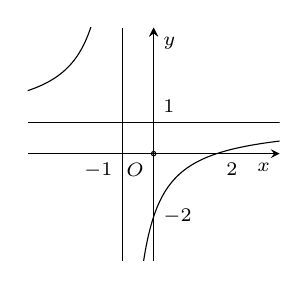
\begin{tikzpicture}[>=stealth,scale=0.4]
		\clip  (-4,-3.4) rectangle (4,4);
		\draw[->,color=black] (-4,0.) -- (4,0.); 
		\foreach \x in  {1,2}
		\draw[->,color=black]  (0.,-4) -- (0.,4);
		 \draw (-1,-4)--(-1,4)
			 (-4,1)--(4,1);
		\draw[smooth,samples=100,domain=-4.5:-1.05] plot (\x,{(\x-2)/(\x+1)}); 
		 \draw[smooth,samples=100,domain=-0.95:4.5] plot (\x,{(\x-2)/(\x+1)});
		\draw  (0,1) node[above right] {\scriptsize $1$};
		\draw  (-1,0) node[below left] {\scriptsize $-1$};
		\draw (0,-2) node[right]  {\scriptsize $-2$};
		\draw (2,0)  node[below right] {\scriptsize $2$};
		\draw (4,0) node[below  left] {\scriptsize $x$};
		\draw (0,4)  node[below right] {\scriptsize $y$};
		\draw (0,0) circle (2pt) node[below  left] {\scriptsize $O$};
	\end{tikzpicture}
			 }
			{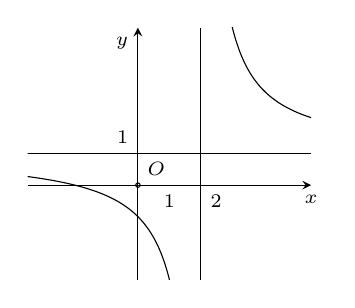
\begin{tikzpicture}[>=stealth,scale=0.4]
		 \clip (-3.5,-3) rectangle (6,5);
		\draw[->,color=black] (-3.5,0.) --  (5.5,0.);
		\draw[->,color=black] (0.,-5) --  (0.,5);
		 \draw (2,-5)--(2,5)
			 (-5,1)--(5.5,1);
		\draw[smooth,samples=100,domain=-4.5:1.9] plot (\x,{(\x+2)/(\x-2)}); 
		 \draw[smooth,samples=100,domain=2.1:5.5] plot (\x,{(\x+2)/(\x-2)});
		\draw  (0,1) node[above left] {\scriptsize $1$};
		\draw (1,0) node[below] {\scriptsize  $1$};
		\draw (2,0)  node[below right] {\scriptsize $2$};
		\draw  (5.5,0) node[below] {\scriptsize $x$};
		\draw (0,4.5) node[left]  {\scriptsize $y$};
		\draw (0,0) circle (2pt)  node[above right] {\scriptsize $O$};
	\end{tikzpicture}
			} 
	 \loigiai{
		Đồ thị của  hàm số đã cho có đường tiệm cận đứng là đường thẳng $x=-1$, tiệm cận ngang là đường thẳng $y=1$ và đi qua các điểm $(0;-2),(2;0)$.}
	\end{ex}

% nguồn: Phan1_Lop_12_Dai_so_Chuong_1
\begin{ex}%[2D1H5-7]%[ma:94d7d395]
	\immini{Đường  cong sau đây là đồ thị hàm số nào?
	\choice 
			{$y=-x^3-3x+2$} 
			{$y=\dfrac{x-1}{x}$} 
			{\True  $y=\dfrac{-x^2}{x+1}$}
			{$y=x^3+3x-2$}} 
			{\begin{tikzpicture}[line cap=butt,line join=miter,>=stealth,scale=0.5,font=\tiny]
		\tikzset{declare function={xmin=-6.2; xmax=4.8; ymin=-4; ymax=7.8;}, 
			smooth,samples=250} 
		\draw[->] (xmin,0)--(xmax,0)  node[shift={(0:7pt)}]{$ x $};
		\draw[->] (0,ymin)--(0,ymax) node[shift={(90:7pt)}]{$ y  $};
		\fill (0,0)  node[shift={(140:5pt)}]{$O$};
		\clip (xmin,ymin-.7) rectangle (xmax,ymax); 
		\foreach\i in {-2,2}{\draw (\i,1.5pt)--(\i,-1.5pt) node[below]{$\i$};} 
		\foreach\j in  {-2,2,4}{\draw (-1.5pt,\j)--(1.5pt,\j) node[right]{$\j$};}
		\def\f (#1){(-(#1)^2)/((#1)+1)} 
		\def\q (#1){(-(#1)+1)} 
		\def\a{0} 
		 \def\b{-2}
		\pgfmathsetmacro\fa{\f (\a)} 
		 \pgfmathsetmacro\fb{\f (\b)}
		\draw[samples=250] plot[domain=-7.4:-1.1]  (\x,{\f (\x)});
		\draw[samples=250] plot[domain=-0.828:15] (\x,{\f  (\x)});
		 \draw plot [domain=-7.4:7] (\x,{\q (\x)});
		 \draw (-1,ymin)--(-1,ymax) node[sloped,pos=0.9,below] {$x=-1$};
		\foreach\x/\y in  {\a/\fa,\b/\fb}{
			\draw[dashed] (\x,0)|-(0,\y);} 
		\foreach\x/\y in {\a/\fa,\b/\fb}{\fill  (\x,\y) circle (1pt);}
	\end{tikzpicture}
			} 
	\loigiai{Dựa vào hình vẽ, đồ thị hàm số có tiệm cận xiên  nên hàm số cần tìm là
			 $y=\dfrac{-x^2}{x+1}$.
		} 
	\end{ex}

% nguồn: Phan1_Lop_12_Dai_so_Chuong_1
\begin{ex}%[2D1H5-7]%[ma:9a690df6]
		Đồ thị hàm số $y=\dfrac{x-1}{-x+2}$ có tâm  đối xứng là điểm có tọa độ
	\choice 
			{\True $I(2;-1)$} 
			{$I(-2;1)$} 
			{$I(2;1)$} 
			{$I(-2;-1)$} 
	\loigiai{ 
			Tâm đối xứng của đồ thị hàm số $y=\dfrac{x-1}{-x+2}$ là  giao điểm hai tiệm cận của nó.\\
			Mà đồ thị  hàm số có tiệm cận đứng $x=2$ và tiệm cận ngang $y=-1$.\\
			Vậy tọa  độ tâm đối xứng $I(2;-1)$.
		 }
	\end{ex}

% nguồn: Phan1_Lop_12_Dai_so_Chuong_1
\begin{ex}%[2D1H5-7]%[ma:721edcb4]
	\immini{ 
		 Bảng biến thiên ở hình vẽ là của hàm số
	 \choice
			 {\True $ y=\dfrac{x+1}{x-1} $}
			 {$ y=\dfrac{x+2}{x-1} $}
			 {$ y=\dfrac{x+1}{1-x} $}
			{$ y=\dfrac{2x+1}{2x+3} $} 
			}{ 
			
\begin{tikzpicture}
				 \tkzTabInit[nocadre=false,lgt=1.2,espcl=2.5,deltacl=0.6]
					{$x$/0.6,$y'$/0.6,$y$/2} 
					{$-\infty$,$1$,$+\infty$} 
				 \tkzTabLine{,-,d,-,}
				\tkzTabVar{+/$1$,-D+/$-\infty$/$+\infty$,-/$1$} 
			\end{tikzpicture}
			 }
	 \loigiai{
			Đồ thị hàm số có tiệm cận đứng là đường thẳng $ x=1 $, tiệm cận ngang là đường thẳng $ y=1 $ và hàm số nghịch biến  trên mỗi khoảng xác định.\\
			Xét $ y=\dfrac{x+1}{x-1} $ có\\ 
			$ \lim\limits_{x\to -\infty}y=1$;  $\lim\limits_{x\to +\infty}y=1 $ nên đường thẳng $ y=1 $ là tiệm cận ngang.\\
			 $ \lim\limits_{x\to 1^{+}}y=+\infty $; $ \lim\limits_{x\to 1^{-}}y=-\infty $ nên đường thẳng $ x=1 $ là tiệm cận đứng.\\
			Lại có $ y'=-\dfrac{2}{(x-1)^{2}}<0 $  nên $ y=\dfrac{x+1}{x-1} $ nghịch biến trên mỗi khoảng xác định, do đó bảng biến thiên trên là của hàm số $ y=\dfrac{x+1}{x-1} $.
		} 
	\end{ex}

% nguồn: Phan1_Lop_12_Dai_so_Chuong_1
\begin{ex}%[2D1H5-7]%[ma:5d2c304b]
	\immini{Đường cong ở hình bên là đồ  thị của hàm số $y=ax^3+b x^2+cx+d$. Khi đó phương trình $y'=0$
	\choice 
			{có  hai nghiệm $x=0$ và $x=1$}
			{có hai nghiệm  $x=\pm1$}
			{vô nghiệm} 
			{\True có một nghiệm kép $x=1$}}{\begin{tikzpicture}[scale=0.9,>=stealth,font=\footnotesize,line join=round,line cap=round]
		\def\a{1} \def\b{-3} \def\c{3} \def\d{-1} 
		 \def\xmin{-2} \def\xmax{3}
		 \def\ymin{-2} \def\ymax{2}
		 \draw[->] (\xmin,0)--(\xmax,0) node [below]{$x$};
		\draw[->] (0,\ymin)--(0,\ymax) node [left]{$y$}; 
		\node at  (0,0) [below left]{$O$};
		\clip  (\xmin+0.1,\ymin+0.1) rectangle (\xmax-0.5,\ymax-0.1);
		 \draw[smooth,samples=300] plot (\x,{\a*(\x)^3+\b*(\x)^2+\c*(\x)+\d});
		\draw (0,-1)  node[left]{$-1$}circle (1pt)
			(1,0) node[above]{$1$}circle  (1pt);
	\end{tikzpicture}
			 }
	 \loigiai{
			Dựa vào hình dáng đồ thị ta có $y'=0$ có đúng một nghiệm $x=1$. 
		} 
	\end{ex}

% nguồn: Phan1_Lop_12_Dai_so_Chuong_1
\begin{ex}%[2D1H5-7]%[ma:e1382c68]
		Số điểm có toạ độ nguyên trên đồ thị hàm số  $y=\dfrac{2x+4}{x-1}$ là
	 \choice
			{\True $8$} 
			{$7$} 
			{$9$} 
			 {$6$}
	\loigiai{ 
			Ta có $y=2+\dfrac{6}{x-1}$, $y\in \mathbb{Z}\Leftrightarrow  x-1$ là ước nguyên của $6$.
			$$x-1\in \left\{\pm 1; \; \pm 2;\; \pm 3;\pm 6\right\}\Rightarrow x\in \left\{-5; \;-2;\;-1;\;  0;\; 2;\; 3;\; 4;\; 7\right\}.$$
			Vậy có $8$  điểm có toạ độ nguyên trên đồ thị.
		} 
	\end{ex}

% nguồn: Phan1_Lop_12_Dai_so_Chuong_1
\begin{ex}%[2D1H5-7]%[ma:ed88c534]
		Bảng biến thiên sau  là của hàm số
		\begin{center}
			
\begin{tikzpicture}
				\tkzTabInit[nocadre=false,lgt=1.2,espcl=2.5,deltacl=0.6] 
					{$x$ /0.6,$y'$ /0.6,$y$ /2} 
					{$-\infty$,$0$,$2$,$+\infty$} 
				\tkzTabLine{,+,0,-,0,+,} 
				 \tkzTabVar{-/$-\infty$,+/$-1$,-/$-5$,+/$+\infty$}
			\end{tikzpicture}
		\end{center}
	 \choice
			 {$ y=-x^3-3x-2 $}
			 {\True $ y=x^3-3x^2-1 $}
			 {$ y=-x^3+3x^2-2 $}
			 {$ y=-x^3+3x^2-1 $}
	 \loigiai{
			\textbf{Cách 1}: Nhìn vào bảng biến thiên ta thấy $ a > 0 $ nên hàm  số cần tìm là $ y=x^3-3x^2-1 $.\\
			\textbf{Cách 2}: Ta có $  y'=3x^2-6x \Rightarrow y' = 0\Leftrightarrow \hoac{& x=0 \\ & x=2. }$\\
			Bảng  biến thiên
			\begin{center}
				
\begin{tikzpicture}
					\tkzTabInit[nocadre=false,lgt=1.2,espcl=2.5,deltacl=0.6] 
						{$x$ /0.6,$y'$  /0.6,$y$ /2}
						{$-\infty$,$0$,$2$,$+\infty$} 
					\tkzTabLine{,+,0,-,0,+,} 
					\tkzTabVar{-/$-\infty$,+/$-1$,-/$-5$,+/$+\infty$} 
				\end{tikzpicture}
			\end{center}
		 }
	\end{ex}

% nguồn: Phan1_Lop_12_Dai_so_Chuong_1
\begin{ex}%[2D1H5-7]%[ma:56cd8976]
	\immini{Đường cong ở hình bên là đồ thị của hàm  số $y=\dfrac{a x+b}{c x+d}$. Mệnh đề nào dưới đây đúng?
	\choice 
			 {$y'<0$, $\forall x\ne2$}
			{$y'<0$,  $\forall x\ne-1$}
			{$y'>0$, $\forall x\ne 2$} 
			{\True $y'>0$, $\forall  x\ne- 1$}
	}{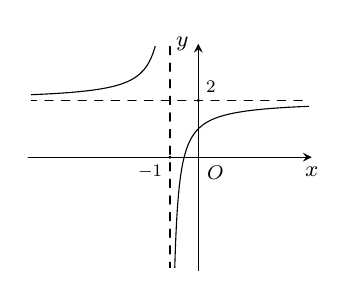
\begin{tikzpicture}[scale=0.6,xscale=0.6,yscale=0.6,>=stealth,font=\footnotesize,line join=round,line cap=round]
		 \def\a{2} \def\b{1} \def\c{1} \def\d{1}
		 \def\xmin{-6} \def\xmax{4}
		 \def\ymin{-4} \def\ymax{4}
		 \draw[->] (\xmin,0)--(\xmax,0) node [below]{$x$};
		\draw[->]  (0,\ymin)--(0,\ymax) node [left]{$y$};
		\node at (0,0)  [below right,scale=0.9]{$O$};
		\clip  (\xmin+0.1,\ymin+0.1) rectangle (\xmax-0.1,\ymax-0.1);
		\draw[smooth,samples=300,domain=\xmin:(-\d/\c-0.1)]  plot (\x,{(\a*(\x)+\b)/(\c*(\x)+\d)});
		 \draw[smooth,samples=300,domain=(-\d/\c+0.1:\xmax)] plot (\x,{(\a*(\x)+\b)/(\c*(\x)+\d)});
		\draw[dashed] (-\d/\c,\ymin)--(-\d/\c,\ymax); 
		\draw[dashed] (\xmin,\a/\c)--(\xmax,\a/\c); 
		\draw (-1,0)  node[below left,scale=0.8]{$-1$}circle (1pt)
			(0,2)  node[above right,scale=0.8]{$2$}circle (1pt);
	\end{tikzpicture}
			 }
	\loigiai{ 
			Dựa vào đồ  thị ta có hàm số đồng biến trên $\mathbb{R}\setminus \{-1\}$ nên $y'>0$, $\forall x\ne- 1$.
		 }
	\end{ex}

% nguồn: Phan1_Lop_12_Dai_so_Chuong_1
\begin{ex}%[2D1H5-7]%[ma:d58836ef]
	\immini{ 
		Một trong bốn điểm sau  đây là tâm đối xứng của đồ thị ở hình bên, điểm đó là điểm nào?
	 \choice
			{$M(1; 2)$} 
			 {\True $N(2; 1)$}
			{$P(1; 0)$} 
			{$Q(0;-1)$} 
			 }{\resizebox{!}{5cm}{
			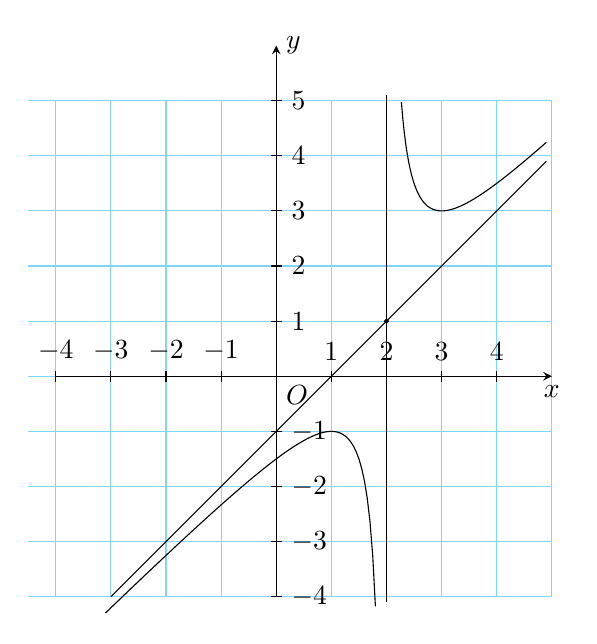
\begin{tikzpicture}[scale=0.7,>=stealth]
				 \draw[cyan!50,thin] (-4.5,-4) grid (5,5);
				\draw[->] (-4,0)--(0,0) 
					node[below right]{$O$}--(5,0) node[below]{$x$}; 
				\draw[->] (0,-4) --(0,6) node[right]{$y$}; 
				 \foreach \x in {-4,-3,-2,-1,1,2,3,4}{
					\draw (\x,-.1)--(\x,.1) node[above]{$\x$}; 
				} 
				 \foreach \y in {-4,-3,-2,-1,1,2,3,4,5}{
					\draw  (-.1,\y)--(.1,\y) node[right]{$\y$};
				 }
				\draw[samples=100,domain=-3.1:1.8] plot  (\x,{(\x)-1+1/(\x-2)});
				\draw[samples=100,domain=2.27:4.9] plot (\x,{(\x)-1+1/(\x-2)}); 
				 \draw [domain=-3:4.9] plot (\x,{(\x-1)});
				\draw  (2,-4.1)--(2,5.1);
				\draw[fill] (2,1) circle (1pt); 
			\end{tikzpicture}
			 }
			 }
	 \loigiai{
			$I$ được gọi là Tâm đối xứng của đồ thị nếu lấy một điểm $A$ thuộc đồ thị sẽ tìm được một điểm $B$ cũng thuộc đồ thị sao cho trung  điểm $AB$ chính là $I$ .\\
			Quan sát hình bên  ta thấy điểm $\mathrm{N}(2; 1)$ là điểm thoả mãn là Tâm đối xứng của đồ thị.\\
			Hoặc ta có thể lấy Tâm đối xứng của đồ thị nếu có giao của $2$ tiệm cận rồi. Áp dụng bài này ta thấy điểm đó  là $\mathrm{N}(2; 1)$.
		} 
	\end{ex}

% nguồn: Phan1_Lop_12_Dai_so_Chuong_1
\begin{ex}%[2D1H5-7]%[ma:bc6bb949]
	\immini{Đồ thị như hình vẽ là của hàm  số
	\choice 
			 {$y=\dfrac{x-1}{-x-1}$}
			{\True  $y=\dfrac{x+1}{x-1}$}
			{$y=\dfrac{x+1}{-x+1}$} 
			 {$y=\dfrac{x-1}{x+1}$}
			}{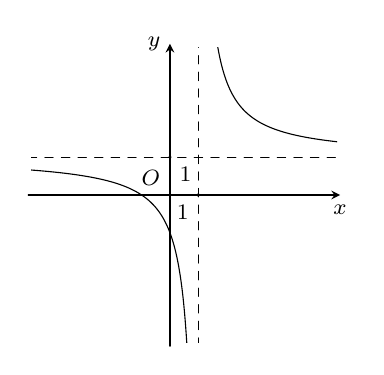
\begin{tikzpicture}[scale=0.6,xscale=0.6,yscale=0.8,>=stealth,font=\footnotesize,line join=round,line cap=round]
		\def\a{1} \def\b{1} \def\c{1} \def\d{-1} 
		\def\xmin{-5}  \def\xmax{6}
		 \def\ymin{-4} \def\ymax{4}
		\draw[->] (\xmin,0)--(\xmax,0) node [below]{$x$}; 
		\draw[->] (0,\ymin)--(0,\ymax)  node [left]{$y$};
		\node  at (0,0) [above left]{$O$};
		\clip (\xmin+0.1,\ymin+0.1)  rectangle (\xmax-0.1,\ymax-0.1);
		\draw[smooth,samples=300,domain=\xmin:(-\d/\c-0.1)] plot (\x,{(\a*(\x)+\b)/(\c*(\x)+\d)}); 
		 \draw[smooth,samples=300,domain=(-\d/\c+0.1:\xmax)] plot (\x,{(\a*(\x)+\b)/(\c*(\x)+\d)});
		\draw[dashed] (-\d/\c,\ymin)--(-\d/\c,\ymax); 
		\draw[dashed]  (\xmin,\a/\c)--(\xmax,\a/\c);
		\draw 
			 (0,1) node[below right]{$1$}circle (1pt)
			(1,0) node[below left]{$1$}circle (1pt); 
	\end{tikzpicture}
			} 
	\loigiai{ 
			Dựa vào đồ thị ta có có tiệm cận đứng là đường thẳng $x=1$ và tiệm cận ngang là  đường thẳng $y=1$ nên hàm số thỏa mãn là $y=\dfrac{x+1}{x-1}$.
		} 
	\end{ex}

% nguồn: Phan1_Lop_12_Dai_so_Chuong_1
\begin{ex}%[2D1H5-7]%[ma:d29bea87]
	 \immini{
		Cho hàm số $y=f(x)$ có đồ thị ở hình bên. Tâm đối  xứng của đồ thị hàm số có toạ độ là
	\choice 
			{\True  $(2;2)$}
			 {$(-2;-2)$}
			{$(-2;2)$} 
			 {$(2;-2)$}
			}{\resizebox{!}{5cm}{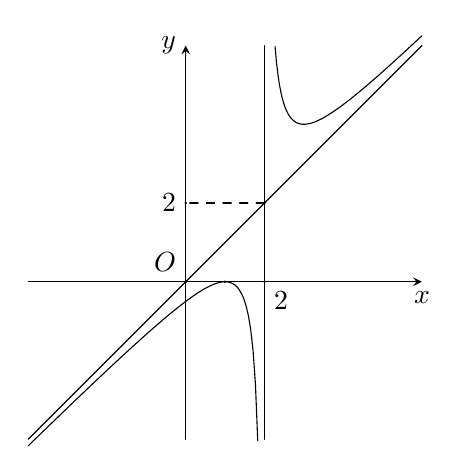
\begin{tikzpicture}[scale=0.5,>=stealth,line join=round,line cap=round]
		\draw[->]  (-4,0)--(6,0) node[below]{$x$};
		\draw[->] (0,-4)--(0,6) node[left]{$y$}; 
		\draw[samples=100,domain=-4:1.83] plot  (\x,{(\x)+1/((\x)-2)});
		\draw[samples=100,domain=2.27:6] plot (\x,{(\x)+1/((\x)-2)}); 
		\draw[samples=100,domain=-4:6] plot (\x,{(\x)}); 
		\draw[samples=100,domain=-4:6,smooth,variable=\y] plot  (2,\y);
		\draw (0,0) node[above  left]{$O$};
		 \draw[dashed]
			 (2,0) node[below right]{$2$}
			(0,2)  node[left]{$2$}
			(2,2)--(0,2); 
		\fill  (2,2) circle (1pt);
		 \fill (0,0) circle (1pt);
		 \fill (1,0) circle (1pt);
		 \fill (2,0) circle (1pt);
		\fill (0,2)  circle (1pt);
	\end{tikzpicture}
			} 
			 }
	 \loigiai{
			Ta có thể quan sát thấy đường thẳng $y=x$ là tiệm cận xiên và $x=2$ là tiệm cận  đứng, giao của chúng là điểm $(2;2)$ nên tâm đối xứng của đồ thị hàm số có toạ độ là $(2;2)$.
		} 
	\end{ex}

% nguồn: Phan1_Lop_12_Dai_so_Chuong_1
\begin{ex}%[2D1H5-7]%[ma:7f6fcda6]
	 \immini{
		Xác định  các hệ số $a, b, c$ để đồ thị hàm số $y=\dfrac{ax-1}{bx+c}$ có đồ thị hàm số như hình vẽ bên là
	 \choice
			 {$a=2,b=2,c=-1$}
			 {$a=2,b=-1,c=1$}
			 {$a=2,b=1,c=1$}
			{\True $a=2,b=1,c=-1$}} 
			{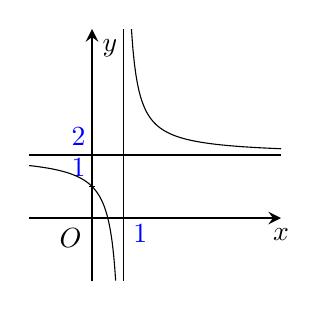
\begin{tikzpicture}[>=stealth,scale=0.4]
		\draw[->,line width = 1pt] (-2,0)--(0,0) node[below left]{$O$}--(6,0)  node[below]{$x$};
		\draw[->,line  width = 1pt] (0,-2) --(0,6) node[below right]{$y$};
		\foreach \x in {1}{\draw  (\x,-.1)--(\x,.1) node[below right,blue]{$\x$};}
		\foreach  \y in {1,2}{\draw[-] (-.1,\y)--(.1,\y) node[above left,blue]{$\y$};}
		\draw plot[domain=-2:0.75,samples=100]  (\x,{((\x)*2-1)/(\x-1)});
		\draw  plot[domain=1.25:6,samples=100] (\x,{((\x)*2-1)/(\x-1)});
		\draw  [domain=-2:6] plot (\x,{2})
			(1,6)--(1,-2); 
	\end{tikzpicture}
			} 
	\loigiai{ 
			 \textbf{Phương pháp:}\\
			Dựa vào đồ thị hàm số để nhận xét và đưa ra công thức đúng về đồ thị hàm số, từ đó  suy ra các giá trị $a, b, c$.\\
			\textbf{Cách  giải:}\\
			Dựa vào đồ thị hàm số ta thấy đồ thị hàm số có tiệm cận ngang là  đường thẳng $y=2\Rightarrow y=\dfrac{a}{b}=2$.\\
			Đồ thị hàm số đi qua điểm $\left(0;1\right)$ nên $-\dfrac{1}{c}=1\Rightarrow  c=-1$.\\
			Mặt khác $-\dfrac  {c}{b}=1\Rightarrow b=1$ suy ra $a=2$.
		} 
	\end{ex}

% nguồn: Phan1_Lop_12_Dai_so_Chuong_1
\begin{ex}%[2D1H5-7]%[ma:8be32ea7]
	 \immini{
		Một trong bốn đường sau đây là một trong hai trục đối xứng của đồ thị ở hình bên, đường  đó là đường nào?
	 \choice
			{$y=-x-1$} 
			{$y=x-1$} 
			 {$y=-x$}
			{\True  $y=x$}
			}{\resizebox{!}{5cm}{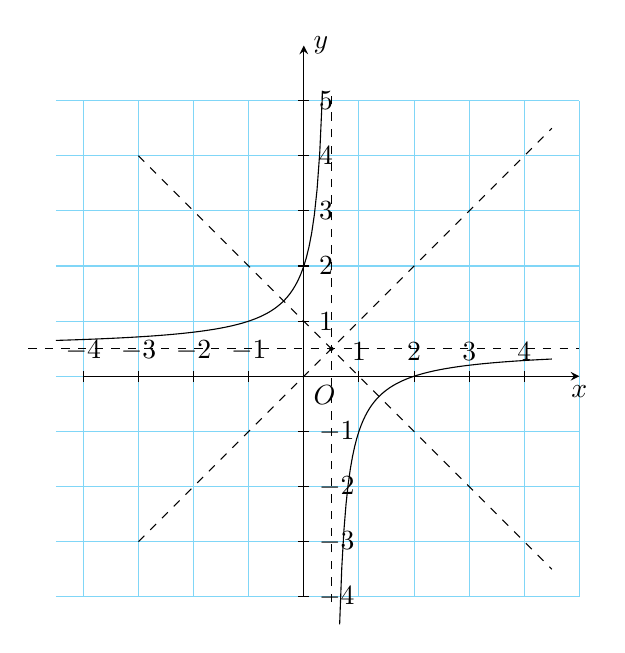
\begin{tikzpicture}[scale=0.7,>=stealth]
		\draw[cyan!50,thin] (-4.5,-4) grid (5,5); 
		\draw[->]  (-4,0)--(0,0)
			node[below  right]{$O$}--(5,0) node[below]{$x$};
		\draw[->] (0,-4)  --(0,6) node[right]{$y$};
		\foreach \x in  {-4,-3,-2,-1,1,2,3,4}{
			\draw (\x,-.1)--(\x,.1) node[above]{$\x$}; 
		} 
		\foreach  \y in {-4,-3,-2,-1,1,2,3,4,5}{
			\draw (-.1,\y)--(.1,\y) node[right]{$\y$}; 
		} 
		\draw[samples=100,domain=-4.5:0.34]  plot (\x,{(\x-2)/(2*(\x)-1)});
		 \draw[samples=100,domain=0.65:4.5] plot (\x,{(\x-2)/(2*(\x)-1)});
		\draw  [domain=-3:4.5,dashed] plot (\x,{(\x)});
		 \draw [dashed] (-5,0.5)--(5,0.5);
		 \draw [domain=-3:4.5,dashed] plot (\x,{(-\x+1)});
		\draw [dashed] (0.5,-4.1)--(0.5,5.1); 
		\draw[fill] (0.5,0.5) circle (1pt); 
	\end{tikzpicture}
			 }
			 }
	 \loigiai{
			$d$ được gọi là Trục đối xứng của đồ thị nếu lấy một điểm $A$  thuộc đồ thị sẽ tìm được một điểm $B$ cũng thuộc đồ thị sao cho $d$ là đường trung trực của $AB$.\\
			Quan sát hình bên ta thấy $y=x$ là đường thẳng thoả mãn  là Trục đối xứng của đồ thị.
		} 
	\end{ex}

% nguồn: Phan1_Lop_12_Dai_so_Chuong_1
\begin{ex}%[2D1V5-7]%[ma:43bde559]
		Đồ thị của hàm số $y=x^3-3mx^2-x+3m$ với $m$ là  tham số đi qua bao nhiêu điểm cố định?
	\choice 
			{$1$} 
			{\True $2$} 
			{$3$} 
			 {$4$}
	 \loigiai{
			Ta có  $y=x^3-3mx^2-x+3m \Leftrightarrow (3x^2-3)m+y-x^3+x=0.$\\
			Phương trình nghiệm đúng với  mọi $m$ khi
			\[\heva{& 3x^2-3=0 \\& y-x^3+x=0}\Leftrightarrow \hoac{& \heva{&  x=1 \\& y=0}\\ & \heva{& x=-1\\& y=0.}} \]
			Đồ thị  hàm số có hai điểm cố định.
		 }
	\end{ex}


%%%%%%%%%%%%%%%% ĐÚNG/SAI %%%%%%%%%%%%%%%%

% nguồn: Phan1_Lop_12_Dai_so_Chuong_1
\begin{ex}%[2D1H5-7]%[ma:5759121d]
	Cho hàm số $y=-\dfrac{-x^2-3x+4}{x-3}$ có đồ thị  là $(C)$.
	\choiceTF 
		 {\True Đồ thị $(C)$ có tiệm cận xiên là $y=-x-6$}
		{\True Đồ thị $(C)$ nhận điểm $I(3; -9)$ làm tâm đối  xứng}
		{\True Đồ thị $(C)$ có hai điểm cực trị nằm  2 phía đối với trục $Oy$}
		{Đồ thị không cắt trục $Ox$} 
	 \loigiai{
		\begin{itemchoice}
			\itemch Tập xác định $\mathscr{D}=\mathbb{R}\setminus\{3\}$.\\ 
			Ta có $y=\dfrac{-x^2-3x+4}{x-3}=-x-6-\dfrac{14}{x-3}$.\\ 
			 Khi đó $\lim\limits_{x \rightarrow+\infty}[f(x)-(-x-6)]=\lim\limits_{x \rightarrow+\infty}\left(-\dfrac{14}{x-3}\right)=0$.\\
			Khi đó đường thẳng  $y=-x-6$ là đường tiệm cận xiên của đồ thị hàm số.
			\itemch Lại có  $\lim\limits_{x\to3^+}f(x)=\lim\limits_{x\to3^+}\dfrac{-x^2-3x+4}{x-3}=-\infty$.\\
			Do đó đồ  thị hàm số nhận đường thẳng $x=3$ là đường tiệm cận đứng.\\
			Suy ra tâm đối xứng là  $I(3;-9)$
			 \itemch Ta có $y'=\dfrac{-x^2+6x+5}{(x-3)^2}=0\Leftrightarrow x^2-6x-5=0\Leftrightarrow\hoac{&x=3+\sqrt{14}\\&x=3-\sqrt{14}.}$\\
			Do đó đồ thị hàm số có hai điểm cực trị nằm  về hai phía của trục tung.\\
			Ta có $y=0\Leftrightarrow  -x^2-3x+4=0\Leftrightarrow\hoac{&x=1\\&x=-4}$.\\
			\itemch Do đó đồ thị hàm số cắt trục $Ox$ tại  hai điểm phân biệt.
		\end{itemchoice}
	} 
\end{ex}

% nguồn: Phan1_Lop_12_Dai_so_Chuong_1
\begin{ex}%[2D1H5-7]%[ma:6261c5b2]
	Cho hàm số $y=\dfrac{2x^2-2x+2}{-x+1}$ có đồ thị  $(C)$.
	 \choiceTF
		{Hàm  số nghịch biến trên khoảng $(-\infty; 0)\cup(2; +\infty)$}
		 {Hàm số đạt cực tiểu tại $x=2$}
		{Giá  trị nhỏ nhất của hàm số trên đoạn $\left[\dfrac{3}{2}; \dfrac{5}{2}\right]$ bằng $-\dfrac{19}{3}$}
		{\True Đồ thị hàm số $(C)$ có tiệm cận xiên là đường  thẳng $2x+y=0$}
	\loigiai{ 
		Tập xác định $\mathscr{D}=\mathbb{R}\setminus\{1\}$.\\ 
		Ta có $y'=\dfrac{-2x^2+4x}{(-x+1)^2}; y'=0\Leftrightarrow  \dfrac{-2x^2+4x}{(-x+1)^2}=0\Leftrightarrow\hoac{&x=0\\&x=2.}$\\
		 Bảng biến thiên
		\begin{center}
			
\begin{tikzpicture}
			\tikzset{double style/.append style={double distance=1.5pt}}
			\tkzTabInit[nocadre=false,lgt=1.2,espcl=2.5,deltacl=0.6] 
				{$x$ /0.6,$y'$ /0.6,$y$  /2}
				 {$-\infty$,$0$,$1$,$2$,$+\infty$}
			\tkzTabLine{,-,$0$,+,d,+,$0$,-,} 
			\tkzTabVar{+/$+\infty$,-/$2$,+D-/$+\infty$/$-\infty$,+/$-6$,-/$-\infty$} 
		\end{tikzpicture}
		\end{center}
		\begin{itemchoice}
			\itemch Hàm số nghịch biến  trên mỗi khoảng $(-\infty; 0)$ và $(2; +\infty)$.
			\itemch Hàm số đạt cực tiểu  tại $x=0$.
			\itemch Giá trị nhỏ nhất của hàm số trên đoạn $\left[\dfrac{3}{2}; \dfrac{5}{2};\right]$ bằng $-7$ tại  $x=\dfrac{3}{2}$.
			\itemch Ta có $\lim\limits_{x\to+\infty}\left[f(x)-(-2x)\right]=\lim\limits_{x\to+\infty}\left[\dfrac{2x^2-2x+2}{-x+1}-(-2x)\right]=\lim\limits_{x\to+\infty}\left(\dfrac{2}{-x+1}\right)=0$.\\ 
			Do đó  đồ thị hàm số có tiệm cận xiên là đường thẳng $y=-2x$.
		\end{itemchoice}
	 }
\end{ex}

% nguồn: Phan1_Lop_12_Dai_so_Chuong_1
\begin{ex}%[2D1H5-7]%[ma:4223a53e]
	Cho hàm số $y=f(x)=\dfrac{x^2-2x+6}{x+1}$  có đồ thị $(C)$. Khi đó
	 \choiceTF
		{\True Hàm số $f(x)$ có  tập xác định là $\mathbb{R}\setminus \{-1\}$}
		{\True Đồ thị $(C)$ có đường tiệm cận  đứng $x=-1$}
		{Tâm đối xứng của đồ thị hàm  số là $I(-1;4)$}
		{\True Trên đồ thị $(C)$ tồn tại đúng $6$ điểm có  tọa độ nguyên}
	 \loigiai{
		\begin{itemchoice}
			 \itemch Đúng.
			\itemch Đúng.\\ 
			Ta có  $\lim\limits_{x\to-1^+} \dfrac{x^2-2x+6}{x+1}=+\infty\Rightarrow x=-1$ là đường tiệm cận đứng.
			\itemch Sai.\\ 
			Ta  có $a=\lim\limits_{x\to+\infty} \dfrac{x^2-2x+6}{x(x+1)}=1$;\\
			$b=\lim\limits_{x\to+\infty} \left(\dfrac{x^2-2x+6}{x+1}-x\right)=\lim\limits_{x\to+\infty}  \dfrac{-3x+6}{x+1}=-3$.\\
			 Tiệm cận xiên của đồ thị hàm số là đường thẳng $y=x-3$.\\
			Đồ thị hàm số có tiệm cận  đứng là đường thẳng $x=-1$ và tiệm cận xiên là đường thẳng $y=x-3$.\\
			Tâm đối xứng của đồ thị  là giao điểm của hai đường tiệm cận là $I(-1;-4)$.
			 \itemch Đúng.\\
			Ta có  $y=f(x)=\dfrac{x^2-2x+6}{x+1}=x-3+\dfrac{9}{x+1}$.\\
			Điểm $M(x;y)\in (C)$ có tọa độ  nguyên thì $\heva{&x\in \mathbb{Z} \\&y\in \mathbb{Z}} \Leftrightarrow \heva{&x\in \mathbb{Z} \\ &9\vdots (x+1).}$\\
			Mà  $9$ có $6$ ước số nên có $6$ điểm có tọa độ nguyên.
		\end{itemchoice}
	} 
\end{ex}

% nguồn: Phan1_Lop_12_Dai_so_Chuong_1
\begin{ex}%[2D1H5-7]%[ma:e1b057ca]
	Cho hàm số  $y=\dfrac{x^2+4x+5}{x+2}$ có đồ thị $(C)$. Khi đó
	\choiceTF 
		 {Hàm số có tập xác định là $\mathscr{D}=\mathbb{R}$}
		 {\True Đồ thị hàm số $(C)$ có tiệm cận xiên là đường thẳng $y=x+2$}
		{\True Đồ  thị hàm số $(C)$ có tiệm cận đứng là đường thẳng $x=-2$}
		{\True Đồ thị hàm số $(C)$ nhận điểm $I(-2; 0)$  làm tâm đối xứng}
	\loigiai{ 
		\begin{itemchoice}
			 \itemch Hàm số có tập xác định là $D=\mathrm{R}\setminus\{-2\}$.
			 \itemch Ta có $y=\dfrac{x^2+4x+5}{x+2}=x+2+\dfrac{1}{x+2}$.
			\begin{itemize}
				\item  $\lim\limits_{x\to+\infty}f(x)=\lim\limits_{x\to+\infty}\left(x+2+\dfrac{1}{x+2}\right)=+\infty$;
				 \item$\lim\limits_{x\to-\infty}f(x)=\lim\limits_{x\to-\infty}\left(x+2+\dfrac{1}{x+2}\right)=-\infty$.
				\item $\lim\limits_{x\to+\infty}\left[f(x)-(x+2)\right]=\lim\limits_{x\to+\infty}\left(\dfrac{1}{x+2}\right)=0$; 
				\item $\lim\limits_{x\to-\infty}\left[f(x)-(x+2)\right]=\lim\limits_{x\to-\infty}\left(\dfrac{1}{x+2}\right)=0$. 
			\end{itemize}
			Do đó  đồ thị hàm số có tiệm cận xiên là đường thẳng $y=x+2$.
			\itemch Ta có 
			\begin{itemize}
				\item $\lim\limits_{x\to-2^+}f(x)=\lim\limits_{x\to-2^+}\left(\dfrac{x^2+4x+5}{x+2}\right)=-\infty$; 
				\item  $\lim\limits_{x\to-2^-}f(x)=\lim\limits_{x\to-2^-}\left(\dfrac{x^2+4x+5}{x+2}\right)=+\infty$.
			\end{itemize}
			Do  đó đồ thị hàm số có tiệm cận đứng là đường thẳng $x=-2$.
			\itemch Đồ  thị hàm số nhận điểm $I(-2; 0)$ làm tâm đối xứng.
		\end{itemchoice}
	} 
\end{ex}

% nguồn: Phan1_Lop_12_Dai_so_Chuong_1
\begin{ex}%[2D1H5-7]%[ma:a5a0c66b]
	Cho hàm số $y=\dfrac{-x^2+x+1}{x+1}$ có  đồ thị $(C)$.
	\choiceTF 
		{\True Hàm số đồng biến trên mỗi khoảng $(-2;  -1)$ và $(-1; 0)$}
		{\True Hàm số có hai điểm  cực trị}
		{Đồ thị $(C)$ không  cắt trục $Ox$}
		{\True Đồ thị $(C)$ có tiệm cận xiên  là đường thẳng đi qua điểm $A(1; 2)$}
	 \loigiai{
		 Tập xác định: $\mathscr{D}=\mathbb{R}\setminus\{-1\}$.\\
		Ta có $y=\dfrac{-x^2+x+1}{x+1}=-x+2-\dfrac{1}{x+1}$ có đạo hàm $y'=\dfrac{-x^2-2x}{(x+1)^2}=0\Leftrightarrow\hoac{&x=0\\&x=-2.}$\\ 
		Bảng  biến thiên:
		\begin{center}
			
\begin{tikzpicture}
			\tikzset{double style/.append style={double distance=1.5pt}}
			\tkzTabInit[nocadre=false,lgt=1.2,espcl=2.5,deltacl=0.6] 
				 {$x$ /0.6,$y'$ /0.6,$y$ /2}
				{$-\infty$,$-2$,$-1$,$0$,$+\infty$} 
			 \tkzTabLine{,-,$0$,+,d,+,$0$,-,}
			\tkzTabVar{+/$+\infty$,-/$5$,+D-/$+\infty$/$-\infty$,+/$1$,-/$-\infty$} 
		\end{tikzpicture}
		\end{center}
		Ta  thấy
		\begin{itemchoice}
			\itemch Hàm số đồng biến  trên mỗi khoảng $(-2; -1)$ và $(-1; 0)$.
			\itemch Hàm số  có hai điểm cực trị.
			 \itemch Ta có $y=0\Leftrightarrow -x^2+x+1=0\Leftrightarrow\hoac{&x=\dfrac{1+\sqrt{5}}{2}\\&x=\dfrac{1-\sqrt{5}}{2}.}$
			Do đó  $(C)$ luôn cắt trục $Ox$ tại hai điểm phân biệt.
			\itemch Đường tiệm cận xiên của đồ thị hàm số là đường thẳng $y=-x+2$ đi qua điểm $A(1; 2)$. 
		\end{itemchoice}
	} 
\end{ex}

% nguồn: Phan1_Lop_12_Dai_so_Chuong_1
\begin{ex}%[2D1V5-7]%[ma:708bb749]
	Cho hàm số $y=\dfrac{-x^2+2(m+1)x-m-5}{x-1}$ có đồ thị $(C)$ với $m$ là tham số 
	\choiceTF 
		 {\True Khi $m=0$ thì đồ thị hàm số có tiệm cận xiên là $y=-x+1$}
		{\True Khi $m=0$ thì  đồ thị hàm số không cắt $Ox$}
		{Để hàm số có cực đại  và cực tiểu thì $m>4$}
		{\True Khi $m=0$, tồn tại $1$  điểm $M$ thuộc đồ thị $(C)$ sao cho $x_M>1$ và độ dài $IM$ ngắn nhất ($I$ là tâm đối xứng của $(C)$). Khi đó tung độ $y_M<-4$}
	 \loigiai{
		\begin{itemchoice}
			\itemch 
			Khi $m=0$  ta có $y=\dfrac{-x^2+2x-5}{x-1}=-x+1-\dfrac{4}{x-1}$.\\
			Tập xác  định $\mathbb{D}=\mathbb{R}\setminus\{1\}$.\\
			$\lim\limits_{x\to\pm\infty}y-(-x+1) = 0$ nên $y=-x+1$ là tiệm cận  xiên.\\
			\itemch Khi $m=0$ ta  có $y=\dfrac{-x^2+2x-5}{x-1}=-x+1-\dfrac{4}{x-1}$.
			Tập xác định  $\mathbb{D}=\mathbb{R}\setminus\{1\}$.\\
			Đạo hàm  $y'=\dfrac{-x^2+2x+3}{(x-1)^2}= 0 \Leftrightarrow -x^2+2x+3=0\Leftrightarrow
			 \heva{&x=-1\Rightarrow y=4.\\&x=3 \Rightarrow y=-4.}$
			Ta có $\lim\limits_{x\to 1^\pm}y=\pm\infty$ nên $x=1$ là đường tiệm cận  đứng;\\
			$\lim\limits_{x\to\pm\infty}y-(-x+1)  = 0$ nên $y=-x+1$ là tiệm cận xiên.
			Đồ thị hàm số không cắt  $Ox$.
			\itemch $y=\dfrac{-x^2+2(m+1)x-m-5}{x-1}$;\\ $y'=\dfrac{-x^2+2x-2m-2+m+5}{(x-1)^2}=\dfrac{-x^2+2x-m+3}{(x-1)^2}$.\\ 
			Hàm số $y$ có cực đại cực tiểu khi  phương trình $-x^2+2x-m+3=0$ có hai nghiệm phân biệt $\Rightarrow\triangle'=1-m+3=4-m>0\Rightarrow m<4$.
			Nghiệm $x=1$ không phải là nghiệm của phương trình  $y'=0\Rightarrow-1+2-m+3\ne 0\Rightarrow m\ne 4$
			Điều kiện sau cùng  $m<4$.
			\itemch $x_M>1\Rightarrow  M$ thuộc nhánh bên phải của $(C)$ và $I$ là tâm đối xứng của $(C)$ nên $I(1;0)$.
			 Toạ độ điểm $M\left(a;-a+1-\dfrac{4}{a-1}\right)$;\\
			 $IM^2=(a-1)^2+\left[(-a+1)^2+\dfrac{16}{(a-1)^2}+8\right]=2(a-1)^2+\dfrac{16}{(a-1)^2}+8$\\
			$IM^2\geq  2\sqrt{2(a-1).\dfrac{16}{(a-1)}}+8\Rightarrow IM^2\ge 8(\sqrt{2}+1)\Rightarrow IM\ge\sqrt{8(\sqrt{2}+1)}$\\
			IM  ngắn nhất khi $$2(a-1)^2=\dfrac{16}{(a-1)^2}\Leftrightarrow(a-1)^4=8\Leftrightarrow a=1+\sqrt[4]8\Rightarrow y_M=-\sqrt[4]8-\dfrac{4}{\sqrt[4]8}<-4.$$
		\end{itemchoice}
	} 
\end{ex}


%%%%%%%%%%%%%%%% TRẢ LỜI NGẮN %%%%%%%%%%%%%%%%

% nguồn: Phan2_Lop_12_Dai_so_Chuong_1
\begin{bt}%[2D1H5-7]%[ma:ec45e922]
	Biết rằng  đường thẳng $y=2x+2m$ luôn cắt đồ thị hàm số $y=\dfrac{x^2+3}{x+1}$ tại hai điểm phân biệt $A, B$ với mọi giá trị của tham số $m$. Hoành độ trung điểm của $AB$ là $x=-m+k$. Giá trị $a$ bằng
	\shortans{-1} 
	\loigiai{ 
		Phương trình hoành độ giao điểm  của $(C)$ và $d$ là:
		$$\dfrac{x^2 + 3}{x+1} = 2x +  2m \Leftrightarrow x^2 + 3 = (2x + 2m)(x+1)$$
		$$\Leftrightarrow x^2 +  3 = 2x^2 + 2x + 2mx + 2m \Leftrightarrow x^2 + 2(1+m)x + 2m - 3 = 0 \quad (1), \quad (x \ne -1).$$
		Đường thẳng $d$ cắt $(C)$ tại hai điểm phân biệt $A, B$ $\Leftrightarrow$ Phương trình (1) có hai nghiệm phân biệt khác $-1$\\ 
		$\Leftrightarrow \begin{cases}
		 \Delta'=(1+m)^2-(2m-3) > 0 \\
		(-1)^2  + 2(1+m)(-1)+2m-3 \ne 0
	\end{cases}
	\Leftrightarrow \begin{cases}
	m^2+2m+1-2m+3>0 \\ 
	1-2-2m+2m-3 \ne 0 
	\end{cases}
	\Leftrightarrow \begin{cases}
	m^2+4>0,\forall m  \\
	 -4 \ne 0
	\end{cases}$
	 Khi đó, gọi $A(x_1;2x_1+2m); B(x_2;2x_2+2m)$.
Hoành độ trung điểm của $AB$ là $x_I=\dfrac{x_1+x_2}{2}=\dfrac{-2-2m}{2}=-m-1$.} 
\end{bt}

% nguồn: Phan2_Lop_12_Dai_so_Chuong_1
\begin{bt}%[2D1V5-7]%[ma:d385169a]
	Một giáo viên theo dõi sự tiến bộ của học sinh qua thang đo điểm, được mô hình hóa bằng hàm số $f(x)=x^3+a x^2+b x+c$ với $a, b, c$  là các hệ số. Trong đó $x(0 \leq x \leq 9, x \in \mathbb{N})$ là số tháng kể từ đầu năm học và $f(x)$ là điểm trong tháng thứ $x$. Qua theo dõi, giáo viên ghi nhận tháng đầu tiên học sinh đạt $19$ điểm, sau đó giảm trong tháng thứ hai và đến tháng thứ ba học sinh đạt mức điểm thấp nhất trong năm học là $3$ điểm. Kể từ tháng thứ ba trở đi, điểm của học sinh tăng lên. Tính điểm của học sinh đó ở tháng thứ sáu.
	\shortans{84} 
	 \loigiai{
		Dựa vào đề bài ta có hệ phương trình: $\left\{\begin{array}{l}f(1)=19 \\ f'(3)=0 \\ f(3)=3
	\end{array} \Leftrightarrow\left\{\begin{array}{l}a+b+c=28 \\ 6 a+b=-27 \\ 9 a+3 b+c=-24
	\end{array} \Leftrightarrow\left\{\begin{array}{l}a=-3 \\ b=-9 \\ c=30
	\end{array}\right.\right.\right.$.
	$$ 
	\Rightarrow f(x)=x^3-3 x^2-9 x+30 \Rightarrow f(6)=84  .
	$$ 
	 }
	\end{bt}

% nguồn: Phan2_Lop_12_Dai_so_Chuong_1
\begin{bt}%[2D1V5-7]%[ma:355d4314]
		Số  điểm có tọa độ nguyên thuộc đồ thị hàm số $y=\dfrac{2x^2+3x+10}{x+2}$ là bao nhiêu?
	\shortans{12} 
	\loigiai{ 
		Ta có: $y=\dfrac{2x^2+3x+10}{x+2}=2x-1+\dfrac{12}{x+2}$\\ 
		Điểm $M(x; y)\in(C)$  có tọa độ nguyên nên
		$\heva{&x \in \mathbb{Z} \\&y \in \mathbb{Z}} \Leftrightarrow\heva{&x  \in \mathbb{Z} \\&12 \ \vdots \ (x+2).}$\\
	Số $12$ có $12$ ước  số nên có $12$ điểm có tọa độ nguyên.}
\end{bt}

% nguồn: Phan2_Lop_12_Dai_so_Chuong_1
\begin{bt}%[2D1V5-7]%[ma:d473384f]
	Tìm được trên đồ thị $(C)\colon y=\dfrac{x^2+4x+5}{x+2}$ hai điểm $M(a;b)$ và $N(c; d)$ có khoảng cách đến đường thẳng $3x+y+6=0$ nhỏ nhất.  Khi đó tính giá trị biểu thức $T=a+b+c+d$.
	\shortans{-4} 
	\loigiai{ 
		 Gọi $M(x_0;y_0)\in(C)\Rightarrow M\left(x_0;\dfrac{x_0^2+4x_0+5}{x_0+2}\right)$.\\
		Gọi $(d)$ là khoảng cách từ $M$ đến  đường thẳng $3x+y+6=0$.\\
		$$d=\dfrac{1}{\sqrt{10}}\left|\dfrac{4x_0^2+16x_0+17}{x_0+2}\right|=\dfrac{1}{\sqrt{10}}\left|4(x_0+2)+\dfrac{1}{x_0+2}\right|\ge\dfrac{4}{\sqrt{10}}.$$ 
		Đẳng thức xảy ra $\Leftrightarrow 4|x_0 + 2| = \dfrac{1}{|x_0 + 2|}  \Leftrightarrow
		\hoac{& x_0 = \dfrac{-3}{2}  \Rightarrow y_0 = \dfrac{5}{2} \\
		&x_0 = \dfrac{-5}{2} \Rightarrow y_0 = \dfrac{-5}{2}.}$\\ 
		Vậy có  hai điểm thoả yêu cầu bài toán là $M_1\left(\dfrac{-3}{2};\dfrac{5}{2}\right)$ và $M_2\left(\dfrac{-5}{2};\dfrac{-5}{2}\right)$.\\
		 Suy ra $T=a+b+c+d=-4$.
	 }
\end{bt}

% nguồn: Phan2_Lop_12_Dai_so_Chuong_1
\begin{bt}%[2D1V5-7]%[ma:df840389]
	Trên đồ thị $(C)\colon \dfrac{x^2-3x+6}{x-2}$ có bao nhiêu cặp điểm đối xứng nhau qua  điểm $I\left(\dfrac{1}{2};1\right)$ ?
	\shortans{2} 
	 \loigiai{
		 Gọi $M(x; y)$; $M'(x'; y')$ thuộc $(C)$ và đối xứng nhau qua điểm $I\left(\dfrac{1}{2};1\right)$.\\
		 Khi đó ta có hệ $\heva{&x+x'=1\\&y+y'=2} \Rightarrow
		\heva{&x'=1-x \\&y'=2-y} \Rightarrow  M'(1-x;2-y)$.\\
		Vì $M(x;y); M'(x'; y')$ thuộc  $(C)$ nên ta có\\
		$\heva{&y = \dfrac{x^2-3x+6}{x-2} \\&2-y=\dfrac{x^2-x+4}{-x-1}}\Rightarrow 2 = \dfrac{x^2-3x+6}{x-2} + \dfrac{x^2+x+4}{-x-1}  \Rightarrow
		\heva{&x^2+x-6=0\\&x\ne-1, x\ne2}\Rightarrow 
		\hoac{&x = -2 \Rightarrow y = -4 \\&x = 3  \Rightarrow y = 6}$\\
	Vậy trên $(C)$ có đúng một  cặp điểm $M(-2,-4)$; $M'(3;6)$}.
\end{bt}


%%%%%%%%%%%%%%%% TỰ LUẬN %%%%%%%%%%%%%%%%

% nguồn: Phan2_Lop_12_Dai_so_Chuong_1
\begin{bt}%[2D1H5-7]%[ma:225ab40b]
	Cho đồ thị hàm số $y=5x-1+\dfrac{8}{x-1}$ có tâm đối xứng $I(a;b)$. Tính giá trị của biểu thức $C=a+3b$. 
	\loigiai{ 
		Hàm số đã cho có tiệm cận đứng là đường thẳng $x=1$ và tiệm cận xiên là đường thẳng $y=5x-1$ nên tâm  đối xứng của đồ thị là $I(1;4)$.\\
		Vậy  $C=a+3b=1+3\cdot 4=13$.
	 }
\end{bt}

% nguồn: Phan2_Lop_12_Dai_so_Chuong_1
\begin{bt}%[2D1V5-7]%[ma:02de6435]
	Cho hàm số $(C_m)\colon  y=\dfrac{x^2+2mx+2}{x+1}=x+2m-1+\dfrac{3-2m}{x+1}$.\\
	Tìm các giá trị của $m$ để hàm số có cực đại, cực tiểu  và khoảng cách giữa hai điểm đó tới đường thẳng $d: x+y+2=0$ bằng nhau.
	\loigiai{ 
		Tập  xác định: $\mathscr{D}=\mathbb{R}\setminus\{-1\}$.\\
		Ta có $y'=\dfrac{x^2+2x+2m-2}{(x+1)^2}$. Khi  đó $y'=0\Leftrightarrow x^2+2x+2m-2=0\, (*)$.\\
		Hàm  số có cực đại và cực tiểu khi và chỉ khi $(*)$ có hai nghiệm phân biệt khác $-1$.\\
		Tương đương $\heva{&\triangle'=3-2m>0\\&(-1)^2+2(-1)+2m-2\neq0}\Leftrightarrow\heva{&m<\dfrac{3}{2}\\&m\neq\dfrac{3}{2}}\Leftrightarrow m<\dfrac{3}{2}$\,  (1).\\
		Gọi $A(x_1; y_1);  B(x_2; y_2)$ lần lượt là hai điểm cực trị của hàm số với $x_1, x_2\neq-1$ là hai nghiệm của phương trình $(*)$.\\
		Áp dụng định lí Vi-et, ta  có $\heva{&x_1+x_2=-2\\&x_1\cdot x_2=2m-2.}$\\
		Mặt khác đường thẳng đi qua  hai điểm cực trị có phương trình là $y=2x+m$ cho nên $y_1=2x_1+m; y_2=2x_2+m\Rightarrow A(x_1; 2x_1+m); B(x_2; 2x_2+m)$.\\
		Theo giả thiết ta có  $\dfrac{|x_1+y_1+2|}{\sqrt{2}}=\dfrac{|x_2+y_2|}{\sqrt{2}}\Rightarrow|x_1+y_1+2|=|x_2+y_2+2|$.\\
		Tương đương 
		\begin{align*}
			&\, |3x_1+2m+2|=|3x_2+2m+2| 
			 \Leftrightarrow (3x_1+2m+2)^2-(3x_2+2m+2)^2=0\\
			 \Leftrightarrow&\, (x_1-x_2)\left[3(x_1+x_2+4m+4)\right]=0\\
			\Leftrightarrow&\, 3(x_1+x_2+4m+4)=0 (x_1\neq x_2)\Leftrightarrow  3(-2+4m+4)=0\\
			\Rightarrow&\, m=-\dfrac{1}{2} \,  \text{ thỏa mãn điều kiện} (*).
		\end{align*}
		Vậy giá trị $m$ cần tìm là  $m=-\dfrac{1}{2}$.
	 }
\end{bt}

% nguồn: Phan2_Lop_12_Dai_so_Chuong_1
\begin{bt}%[2D1C5-7]%[ma:dfc97084]
	Cho hàm số $y=\dfrac{2x-1}{x+1}$ có đồ thị $(C)$. Tính tổng hoành độ của hai điểm nằm  trên $(C)$ đối xứng nhau qua đường thẳng $d:y=3x+5$.
	\loigiai{ 
		Gọi $\Delta$ là  đường thẳng vuông góc với $d$. Khi đó, phương trình $\Delta$ có dạng $y=-\dfrac{1}{3}x+a$.\\
		Phương trình hoành độ giao điểm của (C)  và $\Delta$ là
		\[\dfrac{2x-1}{x+1}=-\dfrac{1}{3}x+a\Leftrightarrow x^{2}+\left( 7-3a \right)x-3-3a=0\ \left( x\neq -1 \right).\tag{1}  \]
		$\Delta$ cắt $(C)$ tại $2$ điểm phân biệt khi $(1)$ có hai nghiệm phân biệt  khác $-1$.
		\[\heva{&\Delta =\left( 7-3a \right)^{2}+12\left( 1+a \right)>0\\&1-\left( 7-3a \right)-3-3a\neq 0}\Leftrightarrow 9a^{2}-30a+61>0\ (\text{đúng với mọi } a).  \]
		Khi đó, $\Delta$ cắt $(C)$ tại hai điểm $A$, $B$  có hoành độ lần lượt là $x_1$, $x_2$ là nghiệm của phương trình (1).\\
		Gọi $M$ là  trung điểm của $AB$, ta có $M\left( \dfrac{x_{1}+x_{2}}{2};-\dfrac{x_{1}+x_{2}}{6}+a\right)$ hay $M\left(\dfrac{3a-7}{2};\dfrac{3a+7}{6} \right)$. \\
		Mặt khác,  $M\in d$ nên $\dfrac{3a+7}{6}=\dfrac{3\left( 3a-7 \right)}{2}+5\Leftrightarrow a=\dfrac{5}{3}$.\\
		Khi đó,  (1) trở thành $x^{2}+2x-8=0\Leftrightarrow x=2$; $x=-4$.\\
		Vậy tổng hoành độ hai điểm thỏa yêu cầu  bằng $2+\left( -4 \right)=-2$.
	} 
\end{bt}
